\chapter{Scene Interpretation}
\label{chp:b4}

In this chapter, we present our mini driverless car's perception capabilities
and how it draws on these capabilities to interpret the current scene into
high-level driving behaviors by means of a rule-based system. We first discuss
our semantic segmentation model and semantic segmentation classes. Second, we
explain the methods we used to locate the right and left lanes with respect to
the body frame. Third, we describe our relatively small classification model
that runs on the top of the segmentation results to classify traffic signs and
lights. Then, we demonstrate our local maps that are used for locating nearby
obstacles. Finally, we introduce our behavior planner, which relates the given
the environmental perception with the traffic rules and picks a primitive
driving pattern accordingly.

\section{Environmental Perception}

\subsection{Semantic Segmentation}

Semantic segmentation is the backbone of our visual perception component. We
deploy a semantic segmentation deep learning model for which we manually
annotate each camera image into ego lane, right lane, left lane, roadside and
traffic sign classes using an image annotation tool, labelme \cite{cite4}. Once
trained, the segmentation model classifies each pixel of the input image into
these classes. In order to visualize the labels, we assign a color for each
class.  Figure \ref{figure:label-visualization} illustrates segmentation labels
blended on the camera images. We annotate traffic lights and traffic signs with
green, ego lane with blue, left lane with yellow, right lane with red, roadside
with pink and all other pixels are considered background and assigned to black
color.

\begin{figure}[h]
  \centering
  \begin{subfigure}[b]{0.4\linewidth}
      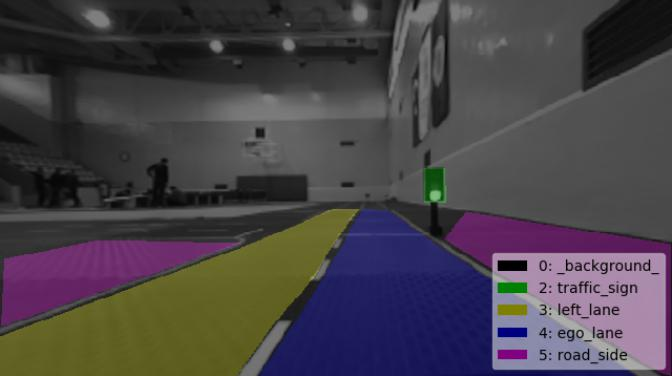
\includegraphics[width=\linewidth]{figures/label-visualization1.jpg}
    \caption{}
  \end{subfigure}
  \begin{subfigure}[b]{0.4\linewidth}
      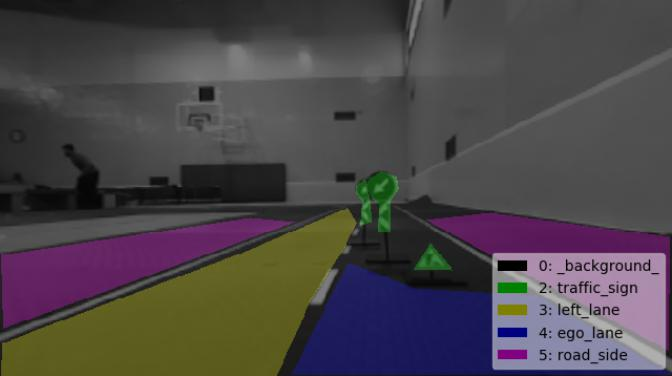
\includegraphics[width=\linewidth]{figures/label-visualization2.jpg}
    \caption{}
  \end{subfigure}
  \begin{subfigure}[b]{0.4\linewidth}
      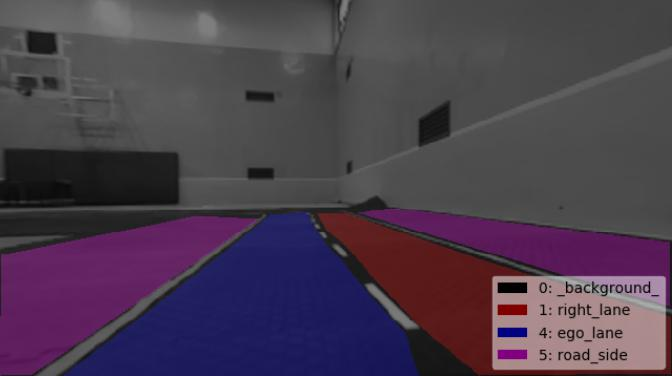
\includegraphics[width=\linewidth]{figures/label-visualization3.jpg}
    \caption{}
  \end{subfigure}
  \begin{subfigure}[b]{0.4\linewidth}
      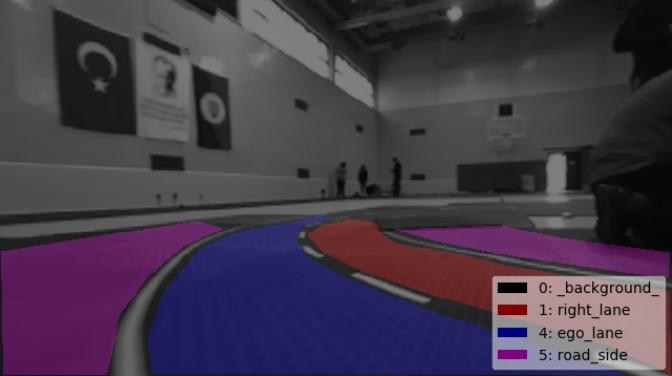
\includegraphics[width=\linewidth]{figures/label-visualization4.jpg}
    \caption{}
  \end{subfigure}
  \caption{(a) Traffic light, ego lane, left lane, and roadside labels. (b)
  Traffic signs, ego lane, left lane, and roadside labels. (c) Ego lane, right
  lane, and roadside labels. (d) Labels on a curvy road segment.}
  \label{figure:label-visualization}
\end{figure}

We adopt U-net architecture for our traffic scene segmentation task inspired
from \cite{cite6}. U-net works well with a few training images and yields fast
and precise segmentations \cite{cite5}. As shown in Figure
\ref{figure:unet-architecture}, the U-net architecture is in shape of U, thus
the name U-net. Our slightly modified architecture inputs an RGB image of size
128x128x3 and encodes it in the contraction side through applying multiple
blocks of layers. Each block takes an input and applies two 3x3 convolutions,
each followed by a batch normalization, ReLU activation, and a 2x2 max pooling
with stride 2 for downsampling. After each downsampling step, we double the
number of feature maps (i.e., the number of filters or channels).  Expansive
side decodes the captured features in the bottleneck section and also is made
of multiple blocks. Each expansive block applies a 2x2 up-convolution for
upsampling, halves the number of feature maps, concatenates the corresponding
feature maps from contracting and expansive sides, and finally applies two 3x3
convolutions, each followed by a batch normalization and ReLU activation. At
the output layer, we use a 1x1 convolution followed by a batch normalization
and softmax to map the resulting 16 feature maps to the desired number of
classes, which is 6 in our case including the background class.

\begin{figure}[h]
  \centering
  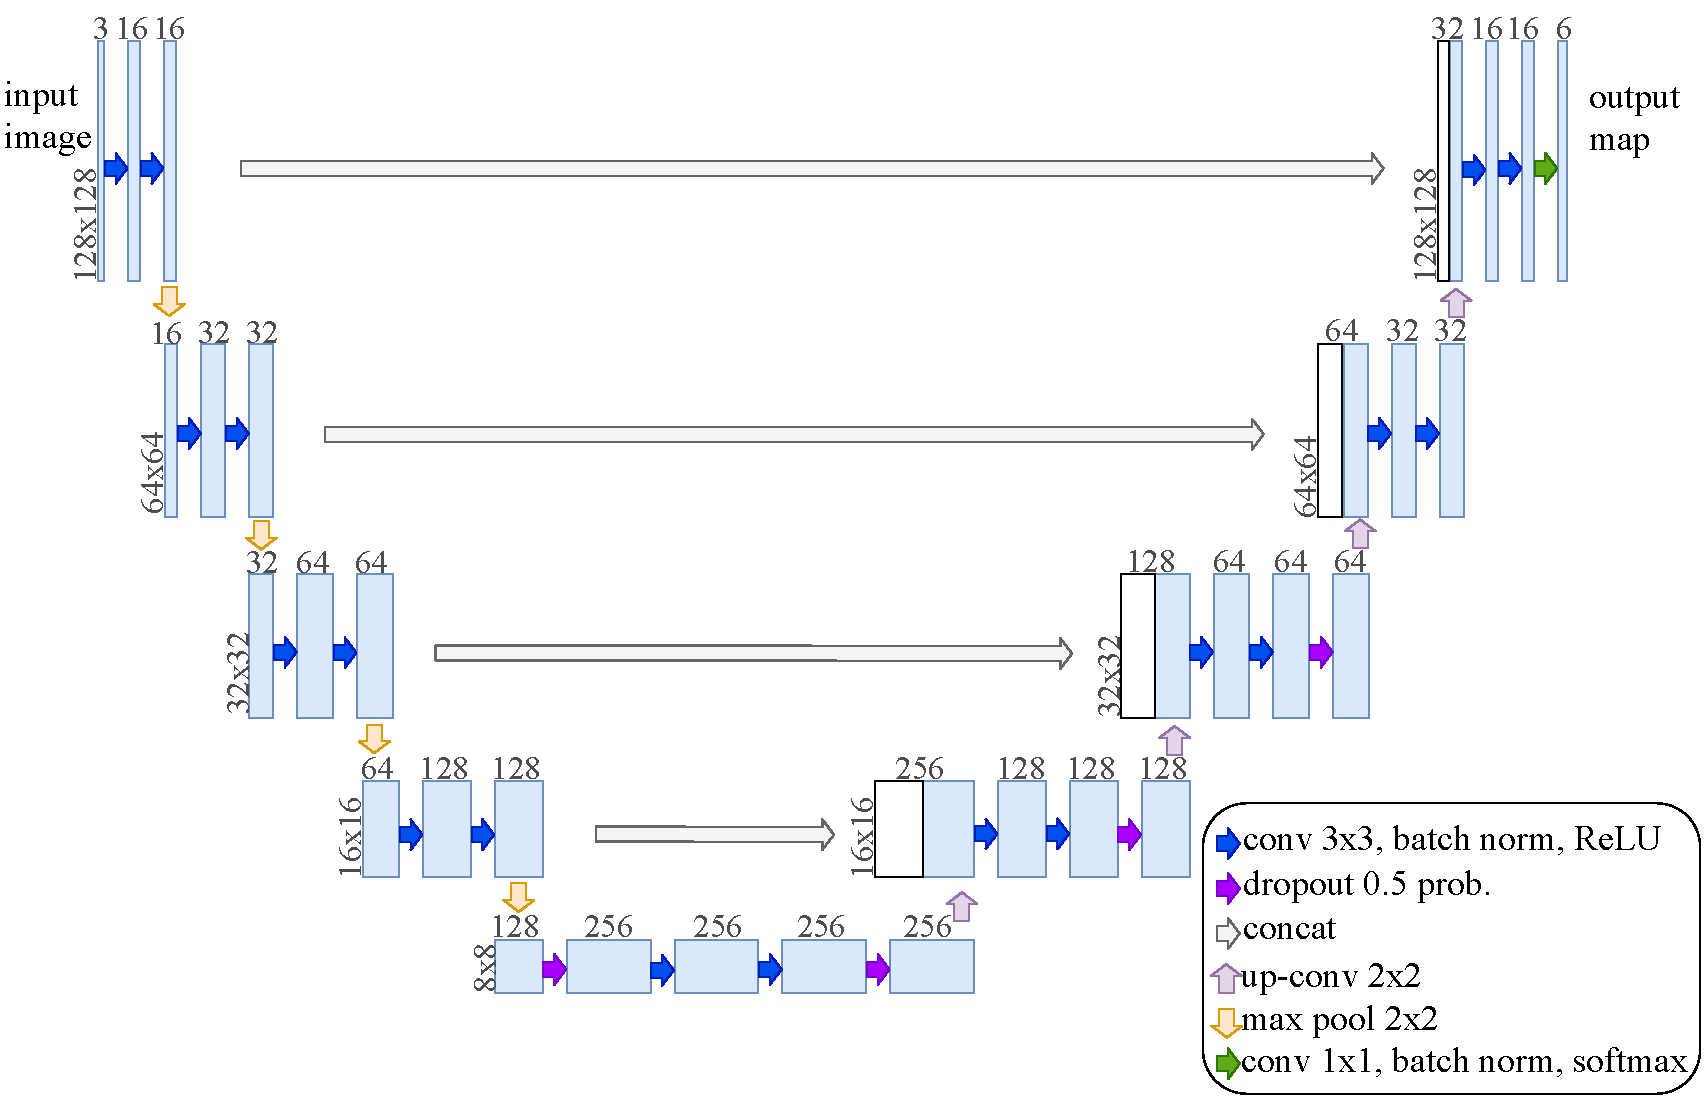
\includegraphics[width=1.0\textwidth]{figures/unet-architecture.pdf}
  \caption{Modified U-net architecture for semantic segmentation. Each blue box
  corresponds to a multi-channel feature map. The number of channels is
  denoted on top of each box. The width x height sizes are provided at the
  lower left edge of each block of layers. White boxes denote the
  concatenated feature maps from the contracting side. The arrows denote
  different operations.}
  \label{figure:unet-architecture}
\end{figure}

In order to meet smooth driving experience requirements, the segmentation
inference shall run at 10 Hz and share the limited resources on the central
computer, which sets an upper bound for the size of our segmentation model.
Therefore, we resize down the camera images from 672x376 to 128x128. We also
lower the initial number of filters to 16, which is 64 in the original U-net
paper. Note that as opposed to the original architecture, we use paddings for
the convolutional layers so that the output of a convolution layer has the same
width and height as the input. As a result, we don't crop contracting feature
maps before concatenating them with the corresponding feature maps on the
expanding side.  Another deviation from the original architecture is that we
train the model in batches(batch size of 8), so we apply batch normalization
following each 3x3 and 1x1 convolutional layers. We also place additional
dropout layers to the bottleneck section and expansive side. We use Adam
optimizer with sparse categorical cross entropy loss function from Keras which
ships with TensorFlow as a high-level API \cite{cite7, cite8}.

\subsection{Lane Detection}

Because we are trying to navigate without a prior map of the environment as in
\cite{cite9}, the lane detection is used not only for adhering to the traffic
rules, but also for the whole navigation task until the car encounters a
traffic sign to change direction.

Our strategy for the lane detection is based on the semantic segmentation. We
first run an argmax on the output segmentation map across the channel axis and
assign a color to each channel as shown in Figure
\ref{figure:label-visualization}. Then we apply inverse perspective mapping to
obtain birdseye view as in Figure \ref{figure:inverse-perspective-mapping}.
The corners of the quadrilaterals in Figure
\ref{figure:inverse-perspective-mapping} are selected such that each pixel in
the birdseye view represents a 1x1 $cm^2$ in the world. Finally, we create a
point cloud from the birdeye view by downsampling it by a factor of 2 for
faster second order polynomial fitting to the lanes. The resultant birdseye
point cloud is also given in Figure \ref{figure:inverse-perspective-mapping}.

\begin{figure}[h]
  \centering
  \begin{subfigure}[b]{0.32\linewidth}
      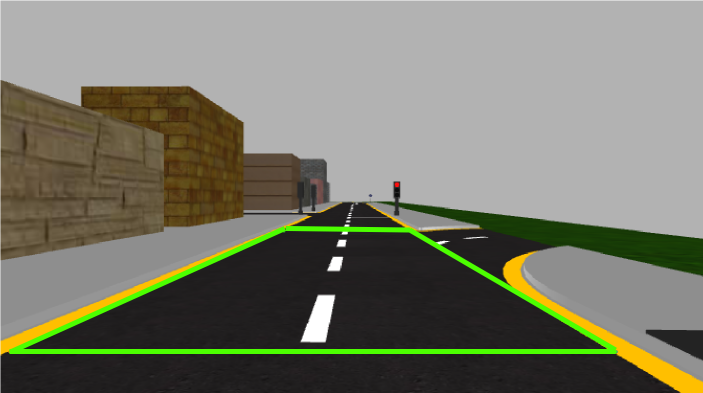
\includegraphics[width=\linewidth]{figures/before-ipm.png}
    \caption{}
  \end{subfigure}
  \begin{subfigure}[b]{0.32\linewidth}
      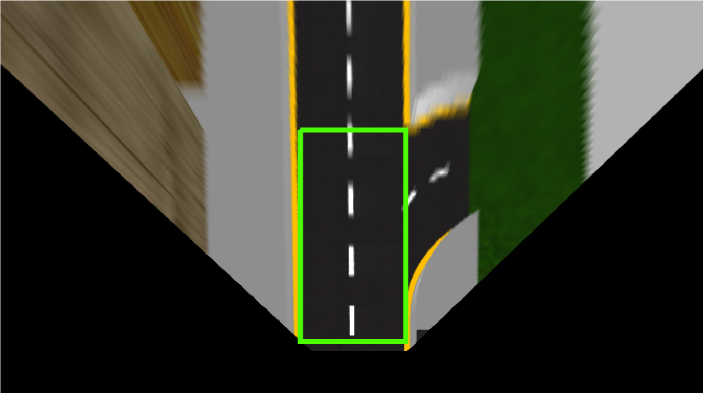
\includegraphics[width=\linewidth]{figures/after-ipm.png}
    \caption{}
  \end{subfigure}
  \begin{subfigure}[b]{0.32\linewidth}
      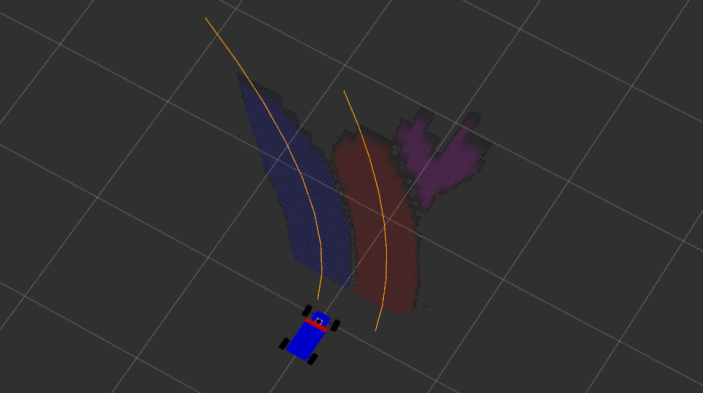
\includegraphics[width=\linewidth]{figures/birdseye-point-cloud.png}
    \caption{}
  \end{subfigure}
  \caption{(a) Before inverse perspective mapping. (b) Birdseye view after
  inverse perspective mapping. (c) Birdseye view point cloud with ego and
  left lane curves in orange.}
      \label{figure:inverse-perspective-mapping}
\end{figure}

In order to find midpoints along the lanes and make it more robust to erroneous
segmentation patches, we apply sliding window and guided searches for each
lane. Both search types are illustrated in Figure \ref{figure:lane-searches}
for the ego lane. It is straightforward to apply the same procedure for the
right and left lanes. While the sliding window search uses histogram to find
starting lane locations, guided search relies on the previous polynomial fits
with some margin. Every time we lose a lane, we initiate a sliding window
search for that particular lane. Once the lane is found, we switch to the
guided search as it is computationally less demanding. For each lane, we
average the coefficients of up to last 5 polynomial fits and obtain the
linearly spaced 9 points along the average polynomial curve. These 9 midpoints
for each lane are the waypoints that describe the lanes on the road.

\begin{figure}[h]
  \centering
  \begin{subfigure}[b]{0.32\linewidth}
      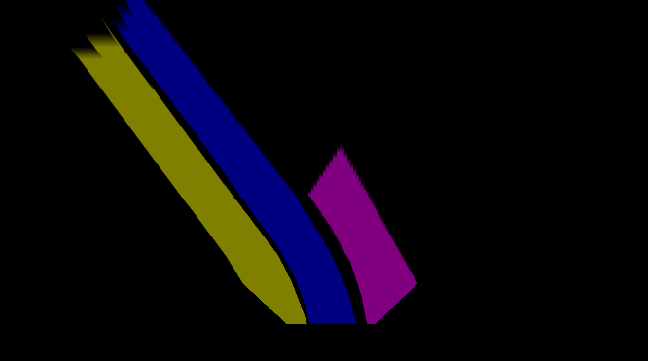
\includegraphics[width=\linewidth]{figures/segmentation-birdseye-view.png}
    \caption{}
  \end{subfigure}
  \begin{subfigure}[b]{0.32\linewidth}
      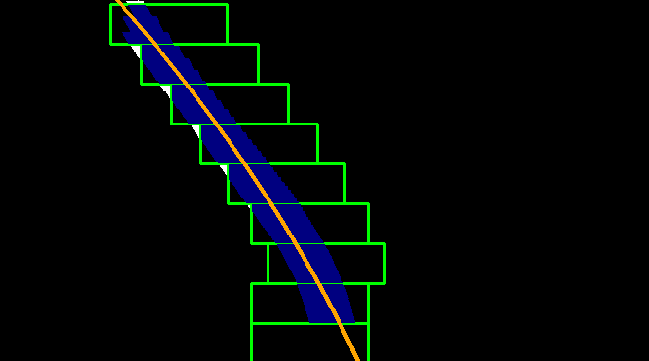
\includegraphics[width=\linewidth]{figures/sliding-window-search.png}
    \caption{}
  \end{subfigure}
  \begin{subfigure}[b]{0.32\linewidth}
      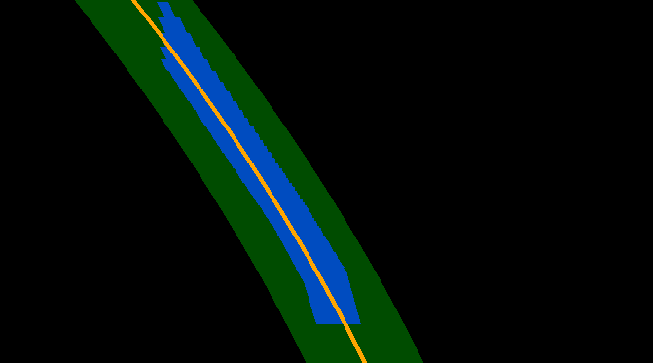
\includegraphics[width=\linewidth]{figures/guided-search.png}
    \caption{}
  \end{subfigure}
  \caption{(a) Segmentation birdseye view image. (b) Sliding window search for
      the ego lane. (c) Guided search for the ego lane on the next image frame
      after the the sliding window search. The green color denotes the sliding
      windows and guided search area. The orange color denotes the averaged
  polynomial curve.}
  \label{figure:lane-searches}
\end{figure}

\subsection{Sign Detection}

Traffic signs and lights regulate the car's behavior on certain conditions and
ensure the car travel the entire course with appropriate direction indications.
We treat the traffic lights the same way as the traffic signs, so the methods
used for the traffic signs also apply to the traffic lights.
O
Though there exist multiple well-established object detection deep learning
architectures with different size, performance and accuracy trade-offs
\cite{cite10}, our limited resources in memory and computational power as well
as the soft realtime requirements at 10 Hz challenges us to use a more
resource-friendly approach. Instead of running an object detection model, we
run a much simpler classifier model on the segmented traffic sign patches. This
approach also saves us from labelling the whole dataset for the object
detection in addition to the semantic segmentation annotations. On the
downside, we can not detect the signs in an end-to-end fasion without resorting
to computer vision techiques for finding bounding rectangles for each sign
patch in the segmentation output \cite{cite13}.

We first create a classification dataset selecting applicable signs from
existing datasets \cite{cite11, cite12}. Because these are small image patches
irrespective of the scene, they worked well for our miniature world. Having
trained the classifier with existing datasets, we run the classifier model
along with the segmentation on our training courses, which contain more traffic
signs than usual. Then, we semi-automatically create a new classification
dataset by cropping and saving the classified traffic sign patches. We later
manually go through the saved image patches and ensure they are in the correct
class folder. Whenever an inappropriate image patch is mistakenly classified as
a traffic sign, we also put them into a special negative class folder.
Augmentating our classification dataset in this manner siginificantly improves
our classifier as it learns from its own mistakes.

We classify \textit{CrossRoad}, \textit{KeepLeft}, \textit{LooseRoad},
\textit{NoEntry}, \textit{Parking}, \textit{ParkingSlot}, \textit{RoadWork},
\textit{StraightOrRight}, \textit{TrafficLightGreen}, \textit{TrafficLightRed},
\textit{TurnLeft}, and \textit{Negative} classes. Figure
\ref{figure:traffic-sign-classes} illustrates these classes with image patches
automatically cropped from the training courses. The paches are converted to
grayscale and resized to 32x32 before fed into the classification model. The
classification architecture is depicted in Figure
\ref{figure:classification-architecture}. We train the model using Adam
optimizer with cross entropy loss in 32 batches applying shift, rescale, shear,
zoom, and brightness augmentation methods from Keras during
training\cite{cite7, cite8}. Algorithm \ref{algorithm:classification} explains
the overall classification process on a traffic sign segmentation mask.

\begin{figure}[h]
  \centering
  \begin{subfigure}[b]{0.15\linewidth}
      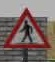
\includegraphics[width=\linewidth]{figures/signs/CrossRoad.jpg}
    \caption{}
  \end{subfigure}
  \begin{subfigure}[b]{0.15\linewidth}
      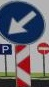
\includegraphics[width=\linewidth]{figures/signs/KeepLeft.jpg}
    \caption{}
  \end{subfigure}
  \begin{subfigure}[b]{0.15\linewidth}
      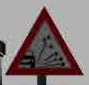
\includegraphics[width=\linewidth]{figures/signs/LooseRoad.jpg}
    \caption{}
  \end{subfigure}
  \begin{subfigure}[b]{0.15\linewidth}
      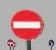
\includegraphics[width=\linewidth]{figures/signs/NoEntry.jpg}
    \caption{}
  \end{subfigure}
  \begin{subfigure}[b]{0.15\linewidth}
      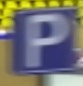
\includegraphics[width=\linewidth]{figures/signs/Parking.jpg}
    \caption{}
  \end{subfigure}
  \begin{subfigure}[b]{0.15\linewidth}
      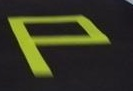
\includegraphics[width=\linewidth]{figures/signs/ParkingSlot.jpg}
    \caption{}
  \end{subfigure}
  \begin{subfigure}[b]{0.15\linewidth}
      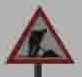
\includegraphics[width=\linewidth]{figures/signs/RoadWork.jpg}
    \caption{}
  \end{subfigure}
  \begin{subfigure}[b]{0.15\linewidth}
      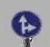
\includegraphics[width=\linewidth]{figures/signs/StraightOrRight.jpg}
    \caption{}
  \end{subfigure}
  \begin{subfigure}[b]{0.15\linewidth}
      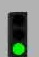
\includegraphics[width=\linewidth]{figures/signs/TrafficLightGreen.jpg}
    \caption{}
  \end{subfigure}
  \begin{subfigure}[b]{0.15\linewidth}
      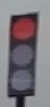
\includegraphics[width=\linewidth]{figures/signs/TrafficLightRed.jpg}
    \caption{}
  \end{subfigure}
  \begin{subfigure}[b]{0.15\linewidth}
      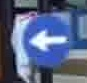
\includegraphics[width=\linewidth]{figures/signs/TurnLeft.jpg}
    \caption{}
  \end{subfigure}
  \begin{subfigure}[b]{0.15\linewidth}
      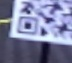
\includegraphics[width=\linewidth]{figures/signs/Negative.jpg}
    \caption{}
  \end{subfigure}
  \caption{Classified and saved traffic sign images from real and simulation
      training courses. (a) CrossRoad, (b) KeepLeft, (c) LooseRoad, (d)
      NoEntry, (e) Parking, (f) ParkingSlot, (g) RoadWork, (h) StraightOrRight,
      (i) TrafficLightGreen, (j) TrafficLightRed, (k) TurnLeft, and (l)
  Negative.} \label{figure:traffic-sign-classes}
\end{figure}

\begin{figure}[h]
  \centering
  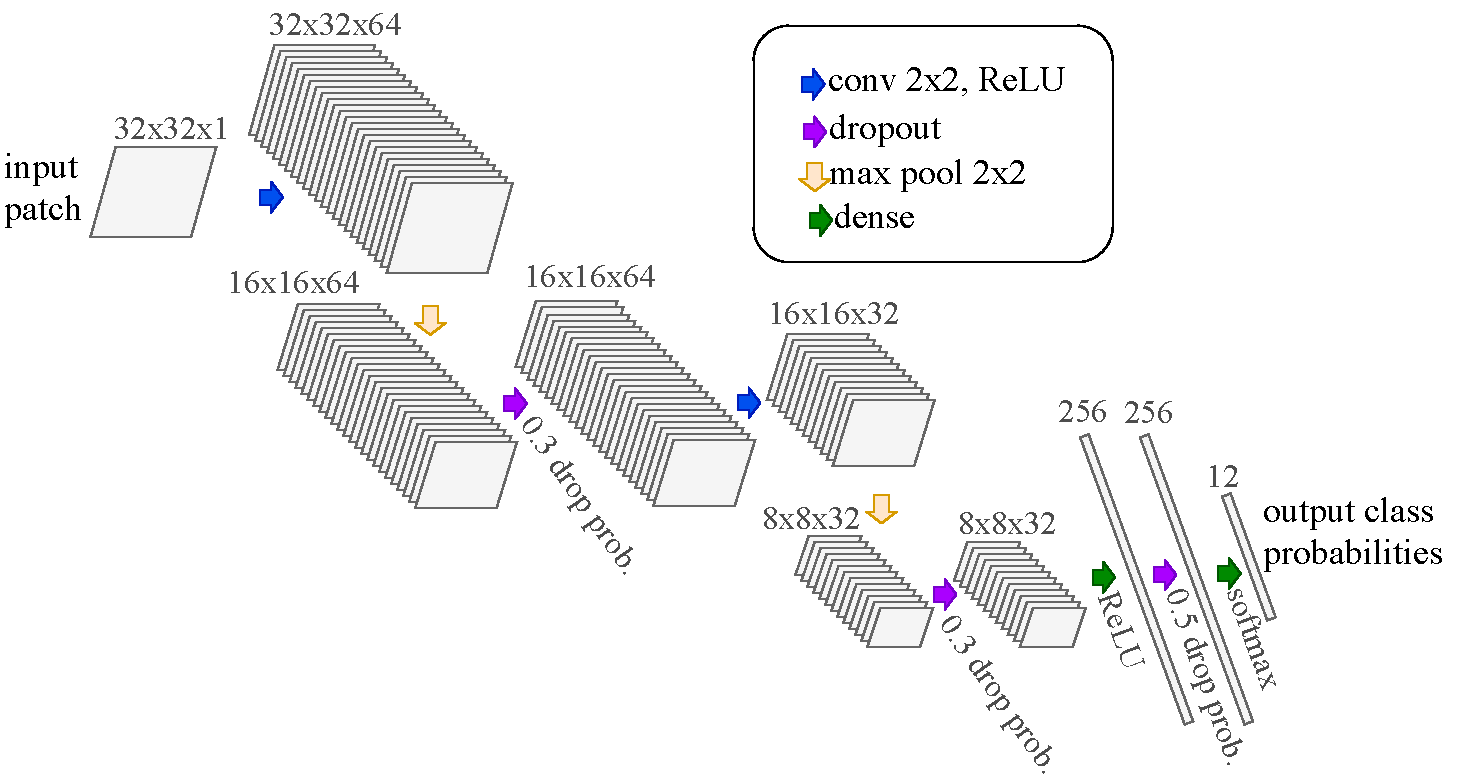
\includegraphics[width=.9\textwidth]{figures/classification-architecture.pdf}
  \caption{Classification architecture. $width \times height\times channel$ is
  given on each layer.}
  \label{figure:classification-architecture}
\end{figure}

\begin{algorithm}[h]
  \caption{Classification of segmented traffic signs.}
  \label{algorithm:classification}
  \begin{algorithmic}[1]
    \Procedure{PARSE-TRAFFIC-SIGNS}{$mask,rgb,depth,intrinsic,record,classes$}
    \State $cx, cy, fx, fy \gets intrinsic$
    \Comment{Unpack camera intrinsic parameters}
    \State $rects \gets list()$
    \State $k \gets 8$
    \Comment{Some pixel margin to the sign patch}
    \State $contours \gets cv2.findContours(mask)$
    \Comment{Use OpenCV to get traffic sign contours}
    \For{$contour$ \textbf{in} $contours$}
      \State $rect \gets cv2.boundingRect(contour)$
      \Comment{Use OpenCV to get a bounding rectangle of each contour}
      \If{$distance(rect, rects[i]) < 32$}
        \State $rects[i] \gets merge(rect, rects[i])$
        \Comment{Merge rectangles if they are too close}
      \EndIf
      \State $rects.append(rect)$
    \EndFor

    \State $t \gets currentTime()$
    \For{$class$ \textbf{in} $classes$}
      \State $events[class] \gets \textbf{False}$
      \If{$t - last(tracks[class]).t > 2$}
        \State \textbf{del} $tracks[class]$
        \Comment{Remove more than 2 second old tracks}
      \EndIf
    \EndFor
      \algstore{classification}
  \end{algorithmic}
\end{algorithm}

\begin{algorithm}
\ContinuedFloat
\caption{Classification of segmented traffic signs (continued)}
  \begin{algorithmic}
    \algrestore{classification}
    \For{$u,v,w,h$ \textbf{in} $rects$}
      \State $sign \gets rgb[v-k:v+h+k, u-k:u+w+k]$
      \State $class, confidance \gets classify(sign)$
      \Comment{Run inference}
      \If{$confidance > 0.8$}
        \State $z \gets mean(depth[v:v+h, u:u+w])$
        \State $x \gets z\frac{u-c_x}{f_x}$
        \State $y \gets z\frac{v-c_y}{f_y}$
        \State $z, x \gets x, z$
        \Comment{Replace x and z for ROS coordinate scheme}
        \State $tracks[class].append(x, y, z, t)$
        \If{$len(tracks[class]) > 3$ \textbf{and} $last(tracks[class]).x < 2.$}
          \Comment{We see the sign more than 3 times with enough confidance within
          a range of 2 meters, so we can safely report that we are tracking it}
          \State $objects[class] \gets (x, y, z, t)$
          \State $events[class] \gets \textbf{True}$
          \If{record \textbf{is True}}
            \State $name \gets unique()$
            \State $save(sign, class, name)$
            \Comment{Record the sign to further enrich the dataset}
          \EndIf
        \EndIf
      \EndIf
    \EndFor
    \State \textbf{return} $tracks, objects, events$
    \EndProcedure
  \end{algorithmic}
\end{algorithm}

\subsection{Obstacle Detection}

We maintain two different local occupancy grids in size and resolution in the
perception component. Each occupancy grid is driven by the same laser scan
message. While 3x3 grid with 0.1 meter/cell resolution is passed to the
trajectory planner, 4x4 grid with 0.2 meter/cell resolution is used to analyze
obstacle in the neighborhood that could change the current driving behavior
such as speed profile, which is also a parameter to the trajectory planner.
Figure \ref{figure:costmaps} demonstrates the local occupancy grids in action.
The car is always centered on the grids; therefore, the grids also move as the
car moves.

\begin{figure}[h]
  \centering
  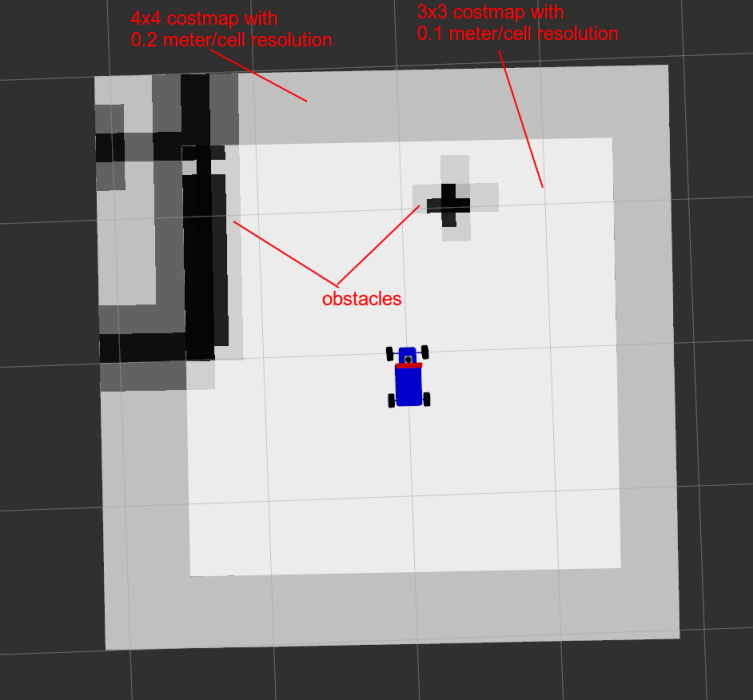
\includegraphics[width=.8\textwidth]{figures/costmaps.png}
  \caption{The small and large local occupancy grids.}
  \label{figure:costmaps}
\end{figure}

We generate two events from the large occupancy grid. The first event,
\textit{ObstacleAhead} indicates there is an obstacle ahead of the car within a
range of 2 meters. The other event, \textit{DangerousObstacle} alerts that
there is an obstacle dangerously too close to the car within 0.7 meters.
Algorithm \ref{algorithm:obstacle-detection} gives the steps for generating
these events.

\begin{algorithm}[h]
  \caption{Obstacle events.}
  \label{algorithm:obstacle-detection}
  \begin{algorithmic}[1]
      \Require Pose $x,y,\theta$ extracted from the latest odometry message.
      $\theta$ is the yaw angle in radian.
      \Procedure{PARSE-OBSTACLES}{$grid,x,y,\theta$}
      \State $nonzeroy, nonzerox \gets nonzero(grid)$
      \Comment{Get nonzero cells (i.e., the obstacle cells)}
      \State $obstaclex \gets nonzerox * grid.resolution + grid.origin.x$
      \State $obstacley \gets nonzeroy * grid.resolution + grid.origin.y$
      \State $diffx, diffy \gets obstaclex - x, obstacley - y$
      \State $angles \gets arctan(\frac{diffy}{diffx})$
      \State $angles \gets rad2deg(\theta - angles)$
      \State $mask = (angles < 10.) \& (angles > -10)$
      \State $events[ObstacleAhead] \gets count\_nonzero(mask) > 0$
      \State $distances \gets \sqrt{diffx^2 + diffy^2}$
      \State $mask = (angles < 10.) \& (angles > -10) \& (distances < 0.7)$
      \State $events[DangerousObstacle] \gets count\_nonzero(mask) > 0$
      \State \textbf{return} $events$
      \EndProcedure
  \end{algorithmic}
\end{algorithm}

\section{Behavior Planning}

Behavior planner consumes the events generated from the perception component.
It transitions the car into appropriate states depending on the hierarchical
finite state machine given in Figure \ref{figure:hfsm} as the events arrive.
When the car is in WAIT state, if there is no obstacle ahead and red light is
not observed, transition 1 is executed and the car starts driving itself. While
the car is moving, if it observes a crossroad sign or a red light, it performs
transition 2 and starts waiting until transition 1 conditions are satisfied. In
DRIVE state, the default behavior is to follow the lanes at normal speed, 0.7
m/s. When the car come across any of straight or turn right, turn left, or park
signs, it stops lane following by sourcing predefined waypoints for these signs
to the trajectory planner instead of the waypoints extracted from the lanes. In
the event that the last predefined waypoint is reached or a manual intervention
through a joystick for an emergency while following a predefined path, runs
transition 4 to put the car back into the lane following state. If any of
LooseRoad, KeepLeft, RoadWork or DangerousObstacle events reported while
driving at the normal speed, the car goes into SLOW SPEED state through
transition 5 and starts driving at 0.5 m/s. When none of these events are
reported, the car switches back to the NORMAL SPEED state. Finally, when the
car sees a parking slot sign on the ground, it performs transition 7 into the
PARK state, in which the car moves into the parking slot and stops.

\begin{figure}[h]
\centering
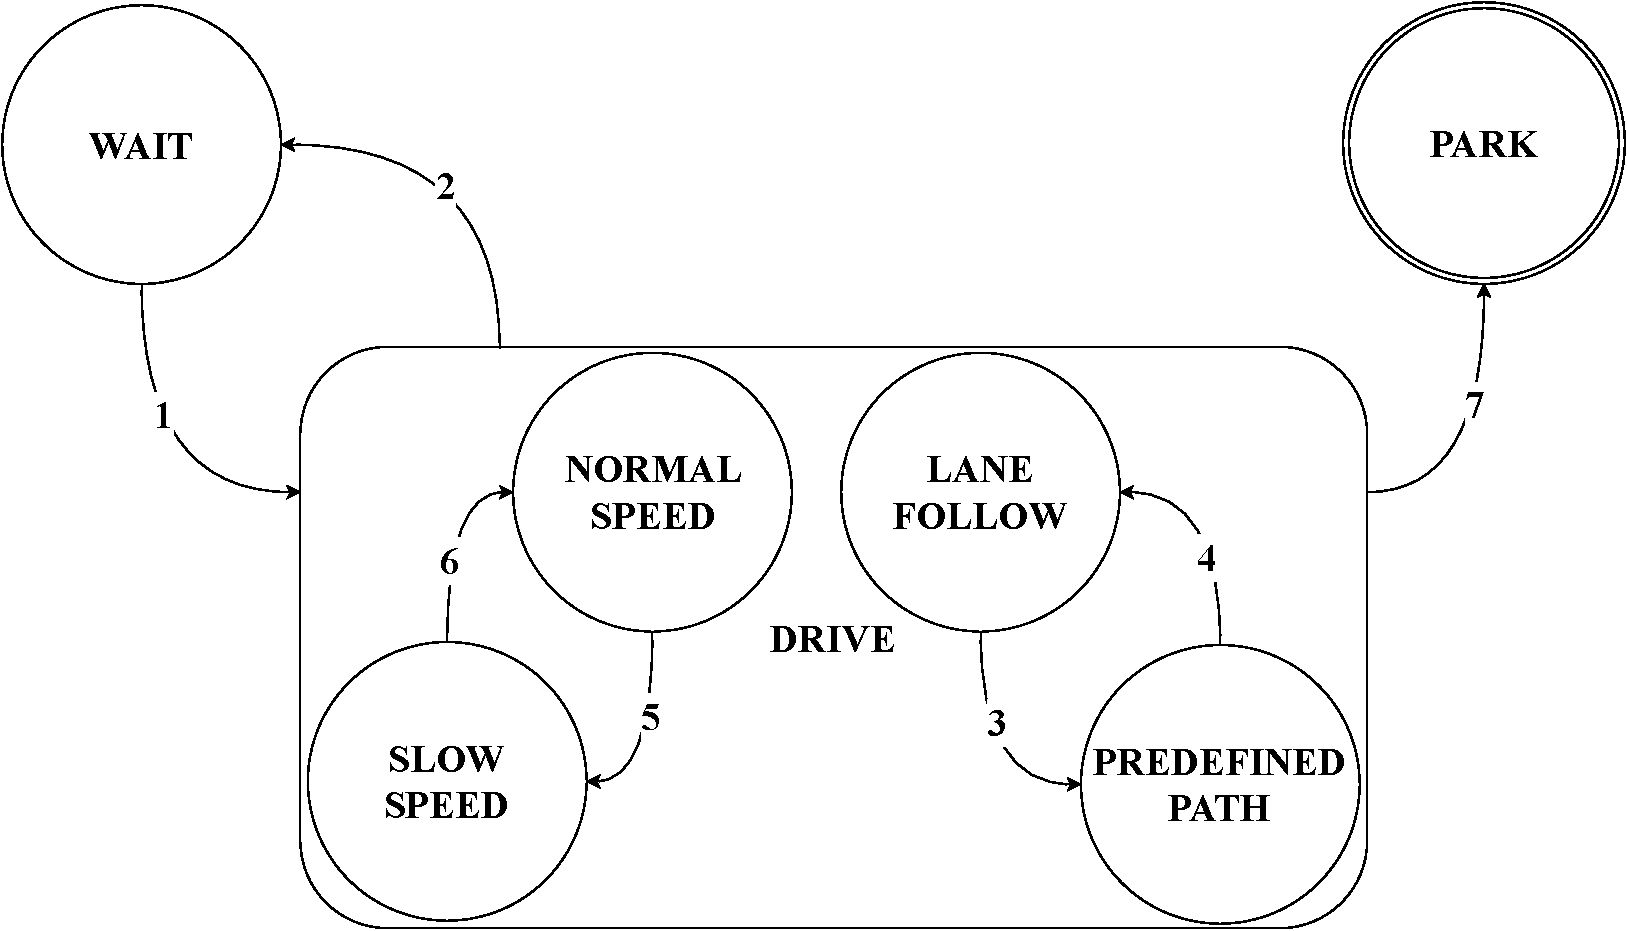
\includegraphics[width=.8\textwidth]{figures/hfsm.pdf}
\caption{Hierarchical finite state machine that governs the high-level behavior
of the car. The numbered arrows 1 to 7 denote the transitions between states.
DRIVE state has two sub-states to control speed profile and waypoint source to
the navigation module. PARK is the terminal state.}
\label{figure:hfsm}
\end{figure}
